\documentclass[useAMS,usenatbib,referee]{biom}
%\usepackage{authblk}
\usepackage{graphicx}
%\usepackage{subcaption}
%\usepackage{float}
\usepackage{amsmath}
%\usepackage{bm}
%\usepackage[authoryear,round, longnamesfirst]{natbib}
%\usepackage{textcomp}
%\usepackage{setspace}
%\usepackage{appendix}
%\doublespacing
%\usepackage{fancyhdr}
\usepackage[]{todonotes}
%\presetkeys{todonotes}{fancyline, color=white}{}
\usepackage{url}

%\pagestyle{fancy}
%\rhead{That's not the Mona Lisa}
%\lhead{}

%\usepackage{geometry}
%\geometry{margin=4cm}

%\usepackage{lineno}
%\linenumbers
%\linespread{1.6}

\title[How to interpret SCR density surface estimates]{That's not the Mona Lisa! How to interpret spatial capture-recapture density surface estimates}

\author{Ian Durbach$^{1,2,*}$, Rishika Chopara$^{3}$, David L. Borchers$^{1,2}$, Rachel Phillip$^{1}$, Koustubh Sharma$^{4}$ \and Ben C. Stevenson$^{3}$ \\
$^{1}$Center for Research into Ecological and Environmental Modelling, \\ School of Mathematics and Statistics, Univeristy of St Andrews, Scotland \\
$^{2}$Center for Statistics in Ecology, the Environment and Conservation, \\ Department of Statistical Sciences, University of Cape Town, South Africa \\
$^{3}$Department of Statistics, University of Auckland, Auckland 1010, New Zealand \\
$^{4}$Snow Leopard Trust, Seattle, Washington, United States of America \\
\email{indurbach@gmail.com}}

\begin{document}

\begin{abstract}
Spatial capture-recapture methods are often used to produce density surfaces, and these surfaces are often misinterpreted. In particular, spatial change in density is confused with spatial change in uncertainty about density. We illustrate correct and incorrect inference visually by treating a greyscale image of the Mona Lisa as an activity center intensity or density surface and simulating spatial capture-recapture survey data from it. Inferences can be drawn about the intensity of the point process generating activity centers, and about the likely locations of activity centers associated with the capture histories obtained from a single survey of a single realization of this process. We show that treating probabilistic predictions of activity center locations as estimates of the intensity of the process results in invalid and misleading ecological inferences, and that predictions are highly dependent on where the detectors are placed and how much survey effort is used. Estimates of the activity center density surface should be obtained by estimating the intensity of a point process model for activity centers. Practitioners should state explicitly whether they are estimating the intensity or making predictions of activity center location, and predictions of activity center locations should not be confused with estimates of the intensity.
\end{abstract}

%because the observation process introduces substantial, spatially-varying uncertainty that distorts any view of density in ways that are impossible to discern from the surface.

\begin{keywords}
Density surface, point processes, spatial capture-recapture.
\end{keywords}

\maketitle 

\section{Introduction}

Spatial capture-recapture (SCR) models \citep*{Efford:04,Borchers+Efford:08, Royle+Young:08} are now widely used to estimate animal abundance and distribution from a variety of data types, including that from camera traps, hair snares, scat surveys, live captures, and acoustic detectors. These methods use the location of the detectors and the locations at which animals were detected (their spatial capture histories) to estimate animal density. The methods have two basic components: a spatial model that quantifies animal activity center (hereafter abbreviated to ``AC'') density at all points in the survey region, and an encounter model that quantifies the expected detection frequency or detection probability, given the AC locations and the detector locations. 

SCR density estimates are often presented graphically in the form of estimated density maps, these being easy to absorb and interpret, at least on the face of it.  However, there are various kinds of density maps that one can produce from SCR analyses and depending on what is presented, it is easy to misinterpret the maps. The most common form of misinterpretation is treating maps that include both spatially varying uncertainty about AC locations and spatially varying AC density estimates as if they were maps of AC density alone. There is also a tendency to refer to densities of animal ACs as densities of {\it animals}. While perhaps done for brevity, lack of clarity invites misinterpretation of maps of AC density as maps of space use -- this is an error because animals distribute themselves around their ACs when they use space, and this is not accounted for in maps of AC density. 

Examples include \cite{Dorazio+Karanth:17}, who say that such maps effectively provide  ``a species distribution model, even in cases where spatial covariates of abundance are unknown or unavailable'', \cite{Alexander+al:15}, who present a map (Figure 4) that includes both spatially varying uncertainty about location and spatially varying AC density and refer to it as the ``spatial distribution of snow leopards'', and \cite{Elliot+Gopalaswamy:16}, who present the same kind of map (Figure 2) and refer to it as the ``pixel-specific lion density''. Minor variations on these themes can be found in many papers, for example ``spatial distribution of the Amur leopard density'' \citep{Qi2015}, ``a pixelated map showing fine-scale variation in density'' \citep{Fouche2020},``spatial variation in the location of estimated activity centers'' \citep{Blanc2013}, ``pixelated SPACECAP leopard density maps'' are used to conclude that ``agricultural land in all three areas is utilized by leopards'' \citep{Devens2021}, ``pixel-specific densities of elephants'' \citep{Goswami2019}, ``a pixelated density map showing relative leopard density \citep{Kandel2020}, ``posterior density estimates for each pixel indicate `density hotspots''' \citep{samarasinghe2022evidence}, ``spatial density estimate of common leopards'' \citep{Goldberg2015}, ``density estimates in home-range centers (number of jaguars per 0.226km$^2$)'' \citep{Lavariega2020}, ``spatial patterns of dhole densities'' \citep{Srivathsa2021}, ``mean posterior density of Amur tiger'' \citep{Xiao2016}, ``modern Bayesian SECR also allows for the computation of area-specific densities and abundance'' \citep{braczkowski2022spatially}, and ``density surface maps can be produced by discretizing the state-space and tallying the number of activity centers occurring in each pixel during each MCMC iteration'' \citep{Chandler+Royle:13}.

The problems with interpretation of such maps arises because (a) uncertainty about the locations of ACs varies spatially, (b) surveys of the same population can produce very different surfaces despite constant AC locations and effort, and (c) there is a failure to clearly distinguish between AC density and usage density.

Misinterpretations arising from (c) are easily avoided if authors clearly specify when they are defining animal density as AC density, or use the term ``AC density'' exclusively. This paper is primarily focused on avoiding misinterpretations arising from ignoring (a) and (b). To do so, we define the two main kinds of densities involved in SCR surveys, and then explain why interpreting one of these as reflecting AC density is nearly always flawed.

\section{Different kinds of density surface}\label{different-densities}

Let us assume that ACs are independently generated by a Poisson process over some region of interest $\mathcal{S}$. Such a process is fully characterized by its intensity function. We could assume that the process is homogeneous, which implies that ACs have independent uniform distributions on $\mathcal{S}$. Alternatively, we can use an inhomogeneous process based on spatially referenced covariates, where the intensity at location $\bm{s}$ is given by $D(\bm{s}|\bm{\beta})=\exp\left\{\beta_0 + \sum_{k=1}^K\beta_kx_k(\bm{s})\right\}$. Here, $\bm{s} \in \mathcal{S}$, $x_k(\bm{s})$ is the $k$th of $K$ covariates evaluated at $\bm{s}$, $\beta_0$ is an intercept parameter, and $\beta_k$ is the slope parameter for the $k$th covariate. We distinguish between two kinds of spatial ``density'' below. 

\subsection{Expected AC density surface} \label{s:eacd}

The first we call the ``expected AC density'' surface. This is $D(\bm{s}|\bm{\beta})$, the intensity function of the underlying point process that is assumed to have generated the ACs. We use the term ``expected'', because the intensity of the point process at $\bm{s}$ is approximately the expected number of ACs per unit area generated by the process in some small region surrounding $\bm{s}$ (and is exactly the expectation as the area of the region approaches zero). This quantity depends only on the parameters of the point process, and is not specific to any particular realization of points. The expected AC density surface can be estimated by $D(\bm{s}|\hat{\bm{\beta}})$, where $\hat{\bm{\beta}}$ is an estimate of $\bm{\beta}$ obtained from a fitted SCR model. Maximum likelihood and Bayesian SCR methods for estimating $\bm{\beta}$ and hence the expected AC density surface are documented in a good number of papers, starting with \cite{Borchers+Efford:08} and \cite{Royle+Young:08}. Both approaches are based on SCR likelihood functions that include a component specifying the AC density surface. 

% The expected number of ACs generated by the process in any region can be calculated by integrating the intensity function over the region. For example, the expected number of activity centers in $\mathcal{S}$ is $\int_{\mathcal{S}} D(\bm{s}|\bm{\beta}) \, d\bm{s}$. 

\subsection{Predicted AC location surface} \label{s:racd}
 
The second surface we call the ``predicted AC location surface''. This is the sum of individual probability densities for the AC locations of capture histories obtained from all detected animals and an estimated number of undetected animals, for whom the capture history is simply no capture at every detector. Each individual AC PDF is a probabilistic prediction, obtained from a fitted SCR model, of where an animal with a particular capture history has its AC. The predicted AC location surface {\it is} a density surface, in that the unit of measurement (defined by the volume under the surface in a region or cell) is ``expected number of ACs'' but, as we show in the remainder of the paper, there are sufficient problems with interpreting the ``expected'' part of it, and enough examples of misinterpretation, that an alternative name that avoids the term ``density'' is preferred. 

%Suppose a single realization of the point process described above has generated $N$ ACs, and that these consistute the animal population to be surveyed. We consider an arbitrary individual $i$ known to exist in the population, and that a survey has resulted in a capture history $\bm{\omega}_i$ for this individual. If $i$ is undetected, the capture history is simply no capture at every detector. 

Given an SCR model with detection function $\bm{\theta}$, the probability $P(\bm{\omega}|\bm{s},\bm{\theta})$ that any potential capture history $\bm{\omega}$ is obtained from an animal whose AC is at $\bm{s}$ can be calculated. Application of Bayes rule gives the probability density that an individual with capture history $\bm{\omega}$ has its AC at $\bm{s}$, $f(\bm{s}|\bm{\omega},\bm{\theta},\bm{\beta})=P(\bm{\omega}|\bm{s},\bm{\theta})f(\bm{s}|\bm{\beta})/\int_{\mathcal{S}} P(\bm{\omega}|\bm{s},\bm{\theta})f(\bm{s}|\bm{\beta})d\bm{s}$, where $f(\bm{s}|\bm{\beta})=D(\bm{s}|\bm{\beta})/\int_{\mathcal{S}} D(\bm{s}|\bm{\beta}) d\bm{s}$ and $D(\bm{s}|\bm{\beta})$ is the intensity function defined above. In the homogenous Poisson case this simplifies to $f(\bm{s}|\bm{\omega},\bm{\theta})=P(\bm{\omega}|\bm{s},\bm{\theta}) /\int_{\mathcal{S}} P(\bm{\omega}|\bm{s},\bm{\theta})d\bm{s}$. We refer to $f(\bm{s}|\bm{\omega},\bm{\theta},\bm{\beta})$ as a probabilistic {\it prediction} for AC location because the prediction can be made for {\it any} capture history, not just those that appear in the data, and because AC location is a random variable, rather than a parameter to be estimated. 

%In practice, a single survey returns a set of capture histories for $n$ animals detected by the survey, $\bm{\Omega}_n=(\bm{\omega}_1, \dots, \bm{\omega}_n)$. Fitting an SCR model to these data provides estimates of detection parameters, $\hat{\bm{\theta}}$, and expected population size, $\hat{N}$. 

%In a maximum likelihood setting predictions are made by substituting the MLE $\hat{\bm{\theta}}$ for $\bm{\theta}$, giving $f(\bm{s}|\bm{\omega},\hat{\bm{\theta}})$. Bayesian methods account for uncertainty in estimates of parameters by considering their entire posterior distribution rather than plugging in point estimates. They choose a prior for $\bm{\theta}$ and compute the posterior density $\pi(\bm{\theta}|\bm{\Omega}_n)$ based on available data $\bm{\Omega}_n=(\bm{\omega}_1, \dots, \bm{\omega}_n)$, the set of capture histories for all $n$ animals detected by the survey, following which a prediction is given by $f(\bm{s}|\bm{\omega})=\int f(\bm{s}|\bm{\omega},\bm{\theta})\pi(\bm{\theta}|\bm{\Omega}_n)\;d\bm{\theta}$. Maximum likelihood and Bayesian SCR methods for estimating the AC PDFs are well documented, for example in Section 4.3 of \cite{Borchers+Efford:08} for maximum likelihood methods and the section ``Estimating derived parameters'' on page 3238 of \cite{Royle+al:09b} for Bayesian methods. If desired, a point prediction may be obtained by taking the mode or expectation of the predicted probability density, though this is rarely done and not considered further here.

In this section we focus on maximum likelihood methods, which make predictions by replacing $\bm{\theta}$ and $\bm{\beta}$ with their MLEs $\hat{\bm{\theta}}$ and $\hat{\bm{\beta}}$, giving $f(\bm{s}|\bm{\omega},\hat{\bm{\theta}},\hat{\bm{\beta}})$. Bayesian methods work similarly but account for uncertainty in estimates of parameters by considering their entire posterior distribution rather than plugging in point estimates. Maximum likelihood and Bayesian SCR methods for computing the individual AC PDFs are well documented, for example in Section 4.3 of \cite{Borchers+Efford:08} for maximum likelihood methods and the section ``Estimating derived parameters'' on page 3238 of \cite{Royle+al:09b} for Bayesian methods. If desired, a point prediction may be obtained e.g.\ by taking the mode of the predicted probability density, though this is rarely done and not considered further here.

The predicted AC location surface $D_p(\bm{s}|\bm{\Omega}_n,\hat{\bm{\theta}},\hat{\bm{\beta}})$ is then defined as the sum of AC PDFs for the capture histories $\bm{\Omega}_n$ of the $n$ animals that were detected by the survey and AC PDFs for the (empty) capture histories $\bm{\omega}=\bm{0}$ of the $\hat{N}_{\bm{0}}$ animals estimated to be present in $\mathcal{S}$ but not detected. Unless there are individual-level covariates that affect detection probability estimates (a complication that we ignore), all undetected animals have the same AC PDF, denoted $f(\bm{s}|\bm{\omega}=\bm{0}, \bm{\theta}, \bm{\beta})$, so that
\begin{equation} \label{eq:pls}
D_p(\bm{s}|\bm{\Omega}_n,\hat{\bm{\theta}},\hat{\bm{\beta}}) = \sum_{i=1}^n f(\bm{s}|\bm{\omega}_i, \hat{\bm{\theta}}, \hat{\bm{\beta}}) + \hat{N}_{\bm{0}} f(\bm{s}|\bm{\omega}=\bm{0}, \hat{\bm{\theta}}, \hat{\bm{\beta}})
\end{equation}
where $\hat{N}_{\bm{0}}=\int_{\mathcal{S}} P(\bm{\omega}=\bm{0}|\bm{s},\hat{\bm{\theta}})D(\bm{s}|\hat{\bm{\beta}}) d\bm{s}$ is the estimated number of undetected animals. Equivalently (see Web Appendix A), the contribution made by undetected animals can be written as $D(\bm{s}|\hat{\bm{\beta}})P(\bm{\omega}=\bm{0}|\bm{s},\hat{\bm{\theta}})$, the formulation used by the R package \texttt{secr}  \citep{secr:22}. It is this surface, usually plotted after discretising the survey region into cells, that many publications (including those listed in the Introduction) interpret as a density surface for AC or animal locations. 

%\begin{equation} \label{eq:pls}
%D_p(\bm{s}|\bm{\Omega}_n,\hat{\bm{\theta}},\hat{\bm{\beta}}) =\sum_{i=1}^n f(\bm{s}|\bm{\omega}_i, \hat{\bm{\theta}}, \hat{\bm{\beta}})+D(\bm{s}|\hat{\bm{\beta}})P(\bm{\omega}=\bm{0}|\bm{s},\hat{\bm{\theta}}) 
%\end{equation}
%Replacing $P(\bm{\omega}=\bm{0}|\bm{s},\hat{\bm{\theta}})$ with $[\int_{\mathcal{S}} P(\bm{\omega}=\bm{0}|\bm{s},\hat{\bm{\theta}})f(\bm{s}|\hat{\bm{\beta}}) d\bm{s}] f(\bm{s}|\bm{\omega}=\bm{0},\hat{\bm{\theta}},\hat{\bm{\beta}})/f(\bm{s}|\hat{\bm{\beta}})$ and $f(\bm{s}|\hat{\bm{\beta}})$ with $D(\bm{s}|\hat{\bm{\beta}})/\int_{\mathcal{S}} D(\bm{s}|\hat{\bm{\beta}}) d\bm{s}$ gives the equivalent form

%\begin{align} \label{eq:pls}
%D_p(\bm{s}|\bm{\Omega}_n,\hat{\bm{\theta}},\hat{\bm{\beta}}) &=\sum_{i=1}^n f(\bm{s}|\bm{\omega}_i, \hat{\bm{\theta}}, \hat{\bm{\beta}})+D(\bm{s}|\hat{\bm{\beta}})P(\bm{\omega}=\bm{0}|\bm{s},\hat{\bm{\theta}}) \\
%&= \sum_{i=1}^n f(\bm{s}|\bm{\omega}_i, \hat{\bm{\theta}}, \hat{\bm{\beta}})+D(\bm{s}|\hat{\bm{\beta}}) \displaystyle\frac{f(\bm{s}|\bm{\omega},\bm{\theta},\bm{\beta})\int_{\mathcal{S}} P(\bm{\omega}|\bm{s},\bm{\theta})f(\bm{s}|\bm{\beta}) d\bm{s}}{f(\bm{s}|\bm{\beta})} \\
%&= \sum_{i=1}^n f(\bm{s}|\bm{\omega}_i, \hat{\bm{\theta}}, \hat{\bm{\beta}}) + \displaystyle\frac{D(\bm{s}|\hat{\bm{\beta}})\int_{\mathcal{S}} D(\bm{s}|\bm{\beta}) d\bm{s}}{D(\bm{s}|\hat{\bm{\beta}}) \int_{\mathcal{S}} D(\bm{s}|\bm{\beta}) d\bm{s}}  \biggl[\int_{\mathcal{S}} P(\bm{\omega}|\bm{s},\bm{\theta})D(\bm{s}|\bm{\beta}) d\bm{s} \biggr] f(\bm{s}|\bm{\omega}=\bm{0}, \hat{\bm{\theta}})
%\end{align}

%The predicted AC location surface $D_p(\bm{s}|\bm{\Omega}_n,\hat{N},\hat{\bm{\theta}})$ is then defined as the sum of AC PDFs for the capture histories $\bm{\Omega}_n$ of the $n$ animals that were detected by the survey and the $\hat{N}-n$ animals that were not detected, where $\hat{N}$ is estimated population size. Unless there are individual-level covariates that affect detection probability estimates (a complication that we ignore), all undetected animals have the same AC PDF, denoted $f(\bm{s}|\bm{\omega}=\bm{0}, \bm{\theta})$, so that
%\begin{equation} \label{eq:pls}
%D_p(\bm{s}|\bm{\Omega}_n,\hat{\bm{\theta}}) =\sum_{i=1}^n f(\bm{s}|\bm{\omega}_i, \hat{\bm{\theta}})+(\hat{N}-n)f(\bm{s}|\bm{\omega}=\bm{0}, \hat{\bm{\theta}}).
%\end{equation}


%While perhaps done for brevity, referring to the predicted AC location surface as an estimated density of {\it animals} (rather than ACs) makes the additional error of ignoring animal movement around ACs. An AC PDF captures only uncertainty about where the AC is located. It is not equivalent to an estimate of the animal's home range and does not provide meaningful information on animal space use --  animals may be present at locations where the predicted AC location surface is close to zero.

%Note that $f(\bm{s}|\bm{\omega},\bm{\theta})$ gives the density of AC locations for a particular capture history $\bm{\omega}$. Doing the survey again can produce a very different prediction. Practically, interpreting the surface as conditional on capture history is not at all straightforward because, as we show in the next section, uncertainty depends on capture history in complicated ways, not all of which are visible on the produced surface. We call this surface a predicted location surface (and explictly avoid calling it a ``density'' surface) to avoid promoting the surface as one that provides meaningful information on AC density.  




% Although this capture history is associated with an individual animal, say $i$, treating it as the density of AC locations for individual $i$ ignores uncertainty in the possible capture histories that might have been obtained. 

%Consider a single individual $i$ known to exist in the population. The location of its AC is a random variable $\bm{S}_i$ with associated probability density $f(\bm{S}_i=\bm{s}_i)$, which we write as $f(\bm{s}_i)$. This density is independent of any data or capture history, but depends only on the underlying point process assumed to generate ACs, and thus can be written as $f(\bm{s}_i|\bm{\beta})$. The exact form of $f$ is not important here but see e.g.\ \citep{Zhang2021}. It follows that all individuals have the same density.


% Suppose now that we conduct a survey. The capture history obtained for individual $i$ is a random variable $\bm{W}_i$ with associated probability density $f(\bm{W}_i=\bm{\omega}_i)$, which we write as $f(\bm{\omega}_i$. If $i$ is undetected, the capture history is simply no capture at every detector. The observed capture history $\bm{\omega}_i$ provides information on where in $\mathcal{S}$ individual $i$'s AC is more likely to be. Given a SCR model with detection function parameters $\bm{\theta}$ and density parameters $\bm{\beta}$, and an observed capture history $\bm{\omega}_i$, the probability density that individual $i$ has its AC at $\bm{s}_i$ is given by $f(\bm{s}_i|\bm{\omega}_i,\bm{\theta},\bm{\beta}$. 

%In a maximum likelihood setting, this density is estimated by $\hat{f}_i=f(\bm{s}|\bm{\omega}_i,\hat{\bm{\theta}})$, where $\hat{\bm{\theta}}$ is the estimate of the detection function parameter vector $\bm{\theta}$ obtained from a fitted SCR model. Bayesian methods for predicted AC location surfaces follow similar principles, but account for uncertainty in estimates of parameters by considering their entire posterior distributions rather than plugging in point estimates. They are constructed using the marginal posterior distribution for each activity centre, $\hat{f}_i=f(\bm{s}|\bm{\omega}_i)=\int f(\bm{s}|\bm{\omega}_i,\bm{\theta})\pi(\bm{\theta}|\bm{\Omega}_n)\;d\bm{\theta}$, where $\pi(\bm{\theta}|\bm{\Omega}_n)$ is the posterior distribution of the parameters given survey data $\bm{\Omega}_n=(\bm{\omega}_1, \dots, \bm{\omega}_n$, the set of capture histories for all $n$ animals detected by the survey. Maximum likelihood and Bayesian SCR methods for estimating the AC PDFs are well documented, for example in Section 4.3 of \cite{Borchers+Efford:08} for maximum likelihood methods and the section ``Estimating derived parameters'' on page 3238 of \cite{Royle+al:09b} for Bayesian methods.

%Note that $f(\bm{s}|\bm{\omega}_i,\hat{\bm{\theta}})$ gives the density of AC locations associated with a capture history $\bm{\omega}_i$, and should not be confused with the density AC locations for individual $i$, which would require marginalising over all possible capture histories. 


%We refer to $\hat{f}_i$ a (probabilistic) prediction for the AC location of individual $i$ because it relates to the outcome of the random variable \bm{S}_i 

%Note that $f(\bm{s}|\bm{\omega}_i,\hat{\bm{\theta}})$ is not a model for the AC location of individual $i$, but only for the AC location of individual $i$ when the capture history is $\bm{\omega}_i$.

%Note that there are three potential sources of uncertainty to account for when predicting an individual's AC location. Firstly, there is uncertainty arising because individual $i$'s capture history is the outcome of a random variable; another survey of the same population might return a very different capture history for individual $i$. Secondly, there is uncertainty arising because the capture histories of all {\it other} individuals are also random; 

%In this section, we will focus on maximum likelihood methods. Bayesian methods for predicted AC location surfaces follow similar principles, but account for uncertainty in estimates of parameters by considering their entire posterior distributions rather than plugging in point estimates. They are constructed using the marginal posterior distribution for each activity centre, $f(\bm{s}|\bm{\omega}_i)=\int f(\bm{s}|\bm{\omega}_i,\bm{\theta})\pi(\bm{\theta}|\bm{\Omega}_n)\;d\bm{\theta}$, found by sampling from the posterior distribution of the parameters. Maximum likelihood and Bayesian SCR methods for estimating the AC PDFs are well documented, for example in Section 4.3 of \cite{Borchers+Efford:08} for maximum likelihood methods and the section ``Estimating derived parameters'' on page 3238 of \cite{Royle+al:09b} for Bayesian methods. 


%The probability density for the location of individual $i$'s AC is given by $f(\bm{s}|\bm{\omega}_i,\bm{\theta})$, where $\bm{\omega}_i$ is the capture history for individual $i$ and $\bm{\theta}$ is the detection function parameter vector. If $i$ is undetected, the capture history is simply no capture at every detector. 

%In a maximum likelihood setting, this density is estimated by $f(\bm{s}|\bm{\omega}_i,\hat{\bm{\theta}})$, where $\hat{\bm{\theta}}$ is the estimate of $\bm{\theta}$ obtained from a fitted SCR model. In this section, we will focus on maximum likelihood methods. Bayesian methods for predicted AC location surfaces follow similar principles, but account for uncertainty in estimates of parameters by considering their entire posterior distributions rather than plugging in point estimates. They are constructed using the marginal posterior distribution for each activity centre, $f(\bm{s}|\bm{\omega}_i)$, found by sampling from the posterior distribution of the parameters. Maximum likelihood and Bayesian SCR methods for estimating the AC PDFs are well documented, for example in Section 4.3 of \cite{Borchers+Efford:08} for maximum likelihood methods and the section ``Estimating derived parameters'' on page 3238 of \cite{Royle+al:09b} for Bayesian methods. 

%Suppose now that the true number of animals in $\mathcal{S}$ is known and denoted by $N$. The predicted AC location surface is defined as the sum of AC PDFs for the $n$ animals that were detected by the survey, and whose capture histories are $\bm{\Omega}_n=(\bm{\omega}_1,\dots,\bm{\omega}_n)$, and the $N-n$ animals that were not detected, whose capture histories are $(\bm{\omega}_{n+1},\dots,\bm{\omega}_{N})=(\bm{0},\dots,\bm{0})$. That is, 
%\begin{equation} \label{eq:pls}
%D_p(\bm{s}|\bm{\Omega}_n,N,\bm{\theta})=\sum_{i=1}^N f(\bm{s}|\bm{\omega}_i, \bm{\theta})
%\end{equation}
%Unless there are individual-level covariates that affect detection probability estimates (a complication that we ignore), all undetected animals have the same AC PDF, denoted $f(\bm{s}|\bm{\omega}=\bm{0}, \bm{\theta})$, and the expression above simplifies to 
%\begin{equation}
%D_p(\bm{s}|N,\bm{\Omega}_n,\bm{\theta})=\sum_{i=1}^n f(\bm{s}|\bm{\omega}_i, \bm{\theta})+(N-n)f(\bm{s}|\bm{\omega}=\bm{0}, \bm{\theta})
%\end{equation}
%
%In reality neither $N$ nor $\bm{\theta}$ are known, and must be estimated from a fitted SCR model. An estimate of the predicted AC location surface is then obtained as 
%\begin{equation}
%\hat{D}_p(\bm{s})=D_p(\bm{s}|\bm{\Omega}_n,\hat{N},\hat{\bm{\theta}}) =\sum_{i=1}^{\hat{N}} f(\bm{s}|\bm{\omega}_i, \hat{\bm{\theta}})=\sum_{i=1}^n f(\bm{s}|\bm{\omega}_i, \hat{\bm{\theta}})+(\hat{N}-n)f(\bm{s}|\bm{\omega}=\bm{0}, \hat{\bm{\theta}})
%\end{equation}

%It is this surface, usually plotted after discretising the survey region into cells, that many publications (including those listed in the Introduction) interpret as a density surface for AC or animal locations. To do so, the estimated number of ACs in a region $\mathcal{A}$ (e.g.\ a cell) is calculated by integrating the estimated predicted location surface over $\mathcal{A}$ i.e.\ $\hat{N}^*_{\mathcal{A}} = \int_{\mathcal{A}} D_r(\bm{s}|\hat{N},\bm{\Omega}_n,\hat{\bm{\theta}}) d\bm{s}$. However, to treat $\hat{N}^*_{\mathcal{A}}$ as an estimate of the true number of ACs in $\mathcal{A}$, $N_{\mathcal{A}}$, is a mistake. Rather, it estimates the integral of the predicted location surface over $\mathcal{A}$, $N^*_{\mathcal{A}}=\int_{\mathcal{A}} D_r(\bm{s}|N,\bm{\Omega}_n, \theta) d\bm{s}$. This is, in contrast to $N_{\mathcal{A}}$, a model-derived quantity of limited biological significance, because it depends on the particular capture history $\bm{\Omega}_n$, which is just one of many possible capture histories that might have been obtained. Estimates are expected to change from survey to survey; estimands are not. Here another survey of the same population of $N$ fixed ACs, with exactly the same sampling intensity, generates a different ``true'' predicted location surface. This makes the surface a poor basis for inference about quantities such as animal densities that are, in reality, fixed. Practically, interpreting the surface as conditional on capture history is not at all straightforward because, as we show in the next section, uncertainty depends on capture history in complicated ways, not all of which are visible on the produced surface. We call this surface a predicted location surface (and explictly avoid calling it a ``density'' surface) to avoid promoting the surface as one that provides meaningful information on AC density.  
%
%While perhaps done for brevity, referring to the predicted AC location surface as an estimated density of {\it animals} (rather than ACs) makes the additional error of ignoring animal movement around ACs. An AC PDF captures only uncertainty about where the AC is located. It is not equivalent to an estimate of the animal's home range and does not provide meaningful information on animal space use --  animals may be present at locations where the predicted AC location surface is close to zero.

\begin{figure}[htbp]
\centering
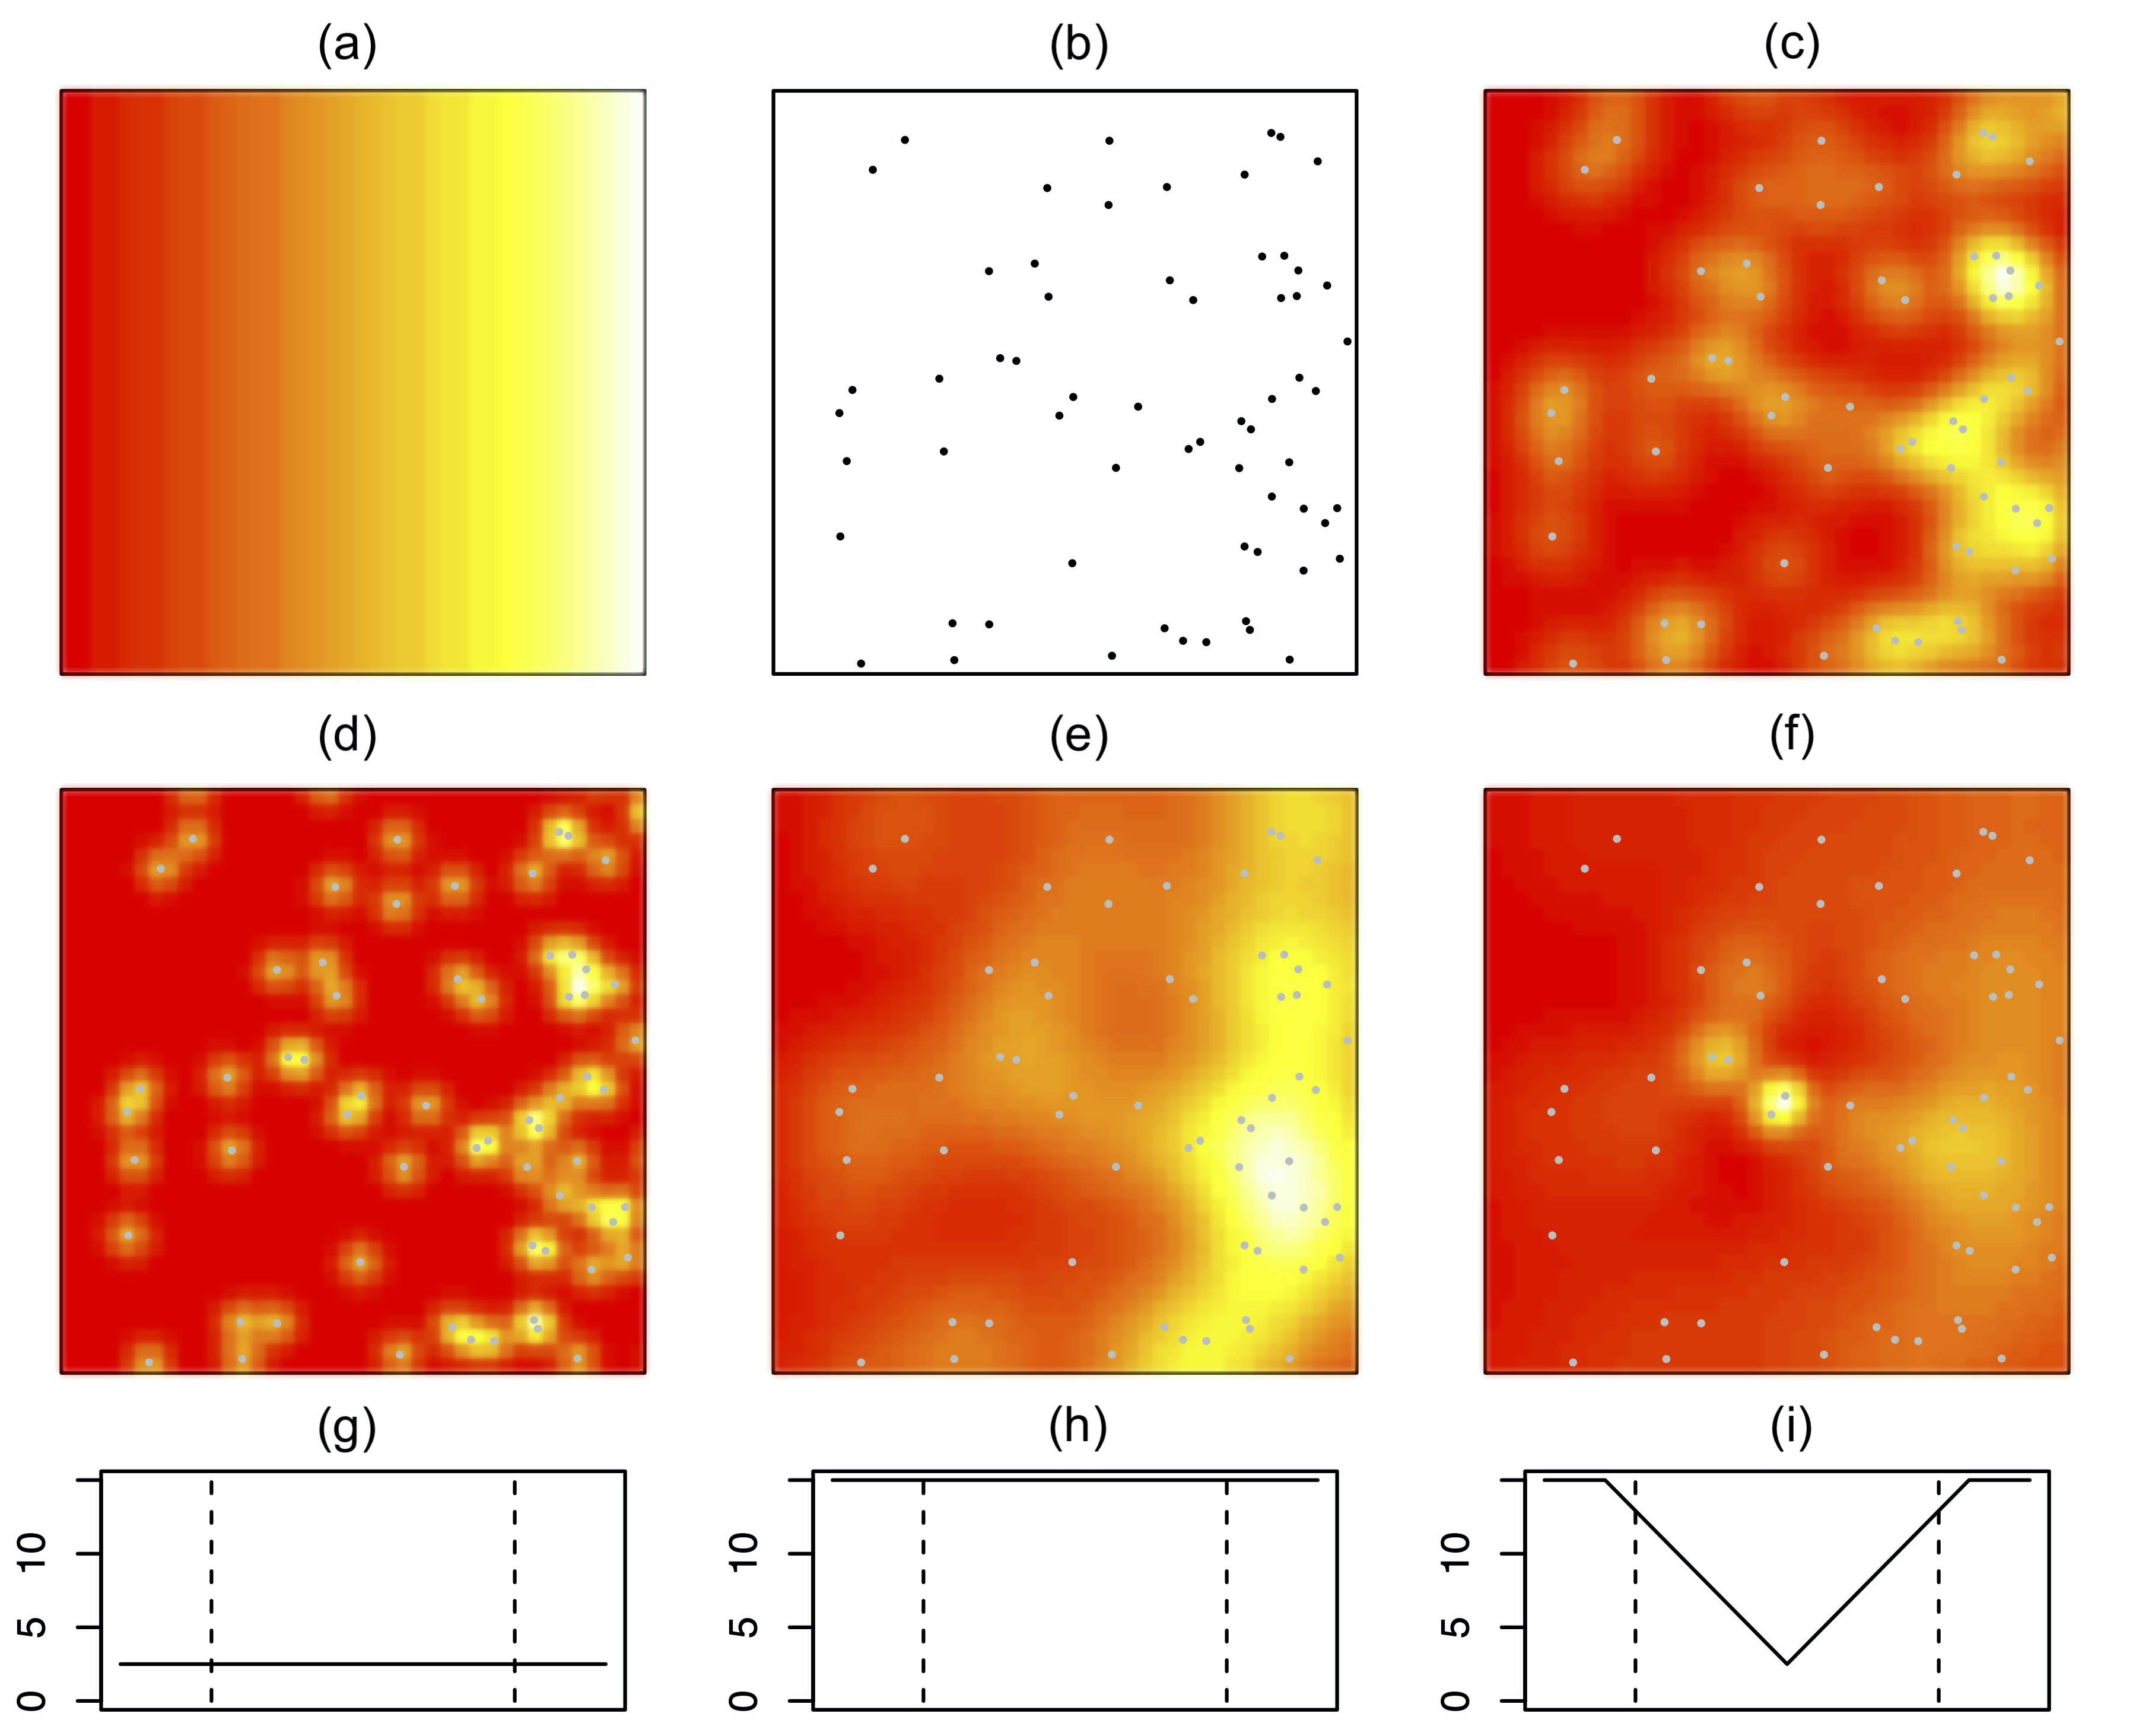
\includegraphics[width=\textwidth]{example-densities.jpg}
\caption{Examples of (a) an AC intensity (density) surface, (b) a realization of ACs from this intensity surface. Panels (c) to (d) show the predicted AC location surface in (b), when the individual AC PDFs ($f_1(\bm{s}),\ldots,f_N(\bm{s})$) are circular bivariate Normal with standard deviations (c) $2.5$, (d) $15$, and (e) $2.5$ for an AC at the center of the plot (dimension 100$\times100$), rising linearly to $15$ by the edge of the plot. True ACs are shown as grey dots. The color scales of panels (c) to (e) are such that the highest and lowest densities in each plot are the same. Panels (f) to (h) plot the standard deviations of the AC PDFs in (c) to (e) against the x-axis. Vertical dashed lines show the extent of the survey region in panels (c) to (e); a buffer beyond this is included because points outside it affect the plot within the survey region. This figure appears in color in the electronic version of this article, and any mention of color refers to that version.}
\label{fig:densities}
\end{figure}

\subsection{Estimated density surfaces}
Figure~\ref{fig:densities} shows examples of both types of surfaces, together with AC locations from a single realization, for a simplified example in which we directly specify the AC PDFs, rather than having to predict them from a fitted model. This allows us to demonstrate our main points while avoiding some of the complexities of SCR surveys (these are addressed in later sections). 

If we are interested in explaining why AC density tends to be high in some places and lower in others, or in characterizing the process that governs the distribution of ACs, then we are primarily interested in estimating a density surface like that shown in Figure~\ref{fig:densities}(a). In this example, it is easting that influences this density, but in general it might be any of a wide variety of habitat or environmental covariates, some of which may be unobserved and evidenced only by spatial clustering of ACs. 

If we are interested only in where the ACs are, and not in explaining why they are there, then Figure~\ref{fig:densities}(b) suffices. We cannot directly observe ACs, but we can obtain individual AC PDFs and sum these to construct a predicted AC location surface using Equation \eqref{eq:pls}. For example, Figure~\ref{fig:densities}(c)-(e) shows predicted AC location surfaces when the individual AC PDFs are bivariate normal distributions with small variance in (c), larger variance in (d), and variance increasing linearly from the center of the plot in (e). The PDFs ``spread'' information about each AC's location according to a bivariate normal distribution, with greater spreading when there is greater uncertainty about location (greater variance).

Ignoring the actual AC dots (because they cannot be observed), Figure~\ref{fig:densities}(c) gives a reasonable visual representation of where the ACs are. It is much more difficult to pick out individual ACs from Figure~\ref{fig:densities}(d), but it gives a reasonable representation of where the high- and low-density regions of ACs are -- much like Figure~\ref{fig:densities}(a), but customized somewhat for this particular realization of AC locations rather than their long-run average locations. Note, however, that these two figures are representations of exactly the same set of ACs and that if one interprets them as plots of AC density, they contradict each other. Figure~\ref{fig:densities}(c) says that almost all the region has low density (red in Figure~\ref{fig:densities}: this figure appears in color in the electronic version of this article, and any mention of color refers to that version) and that there are lots of small high-density regions, while Figure~\ref{fig:densities}(d) says that there is much less variation in density, that there are large swathes of higher density (the yellow towards the right) and large swathes of low density towards the left. The reason that Figure~\ref{fig:densities}(d) shows less variation in density is not that there is less variation in the population (there are exactly the same ACs in both (c) and (d)), it is that we are less sure about the location of the ACs in (d). To interpret this as less variation in AC density is to invite incorrect ecological inferences.

Now what about Figure~\ref{fig:densities}(e)? If this is interpreted as indicating where the high and low-density regions are, it is misleading. It says that the highest density region is in the center of the plot, and that the region with most variation in density is the central region, which is not true. 

The fact that there is only small uncertainty about AC location in the center of the plot and large uncertainty error at the edges means that the ACs near the center are not ``spread'' much and therefore appear as higher peaks in the surface, with low regions where there are no ACs. Near the edges of the plot, on the other hand, uncertainty about AC location is high and ACs are ``spread'' a lot, which both flattens the peaks at individual AC locations and ``fills in'' the troughs where there are no ACs. 

It is a feature of SCR surveys that the AC locations of individuals farther from the detector array tend to be estimated with greater uncertainty than individuals within the array. This is illustrated in Figure~\ref{fig:screrr}, which shows the predicted AC PDFs of two animals detected by two simulated SCR surveys of the same population. With only two animals shown it is clear that the surface largely conveys information about uncertainty in predicted AC locations -- the more spread-out contours in the top left reflects greater uncertainty in the predicted location of one animal's AC, not that fewer animals have their ACs there. This becomes far less easy to see when there are many animals with overlapping AC PDFs. There is also sampling variation in the possible capture histories that might have been obtained for a given animal, which can be substantial and which is not reflected in the predicted AC location surface for a single survey (compare, for example, the AC PDF obtained for animal A in each survey). 

%The reason contours in the top left of the figure ``avoid'' the triangle is because the detection function range, estimated from the whole survey, not just the points shown, is large and if the AC was near the triangle, other detectors would have high probability of detecting it. The fact that they did not makes them ``repel'' the AC. 

\begin{figure}[htbp]
\centering
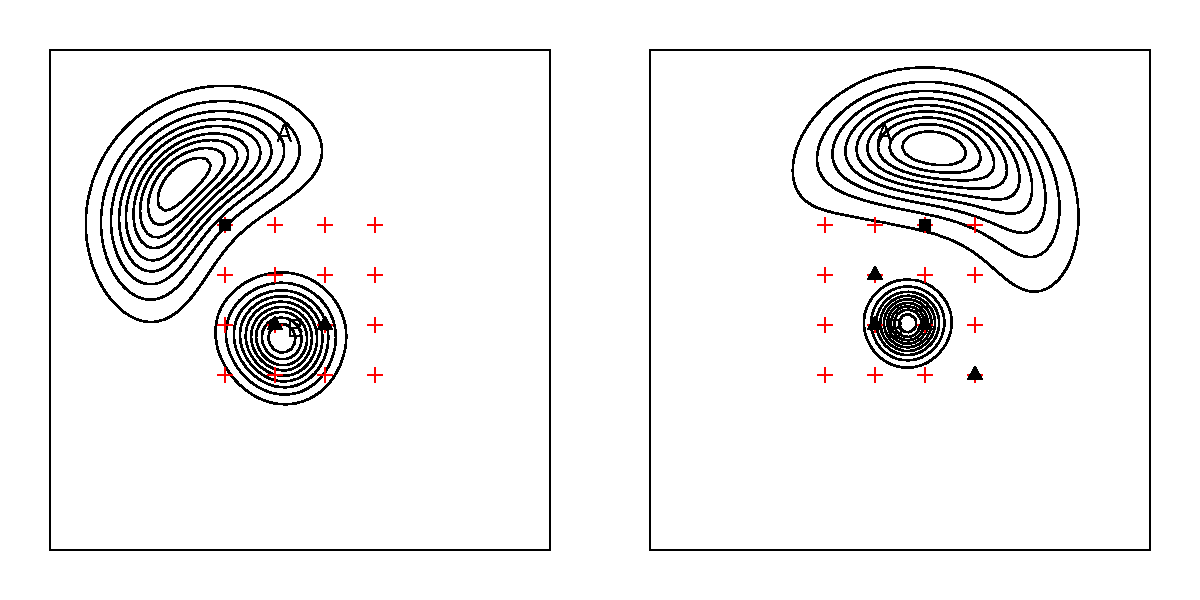
\includegraphics[width=\textwidth]{screrr.pdf}
\caption{Contours of the AC PDFs for two detected individuals in two simulated SCR surveys of the same population. Detectors are shown as crosses. Animal A was detected at detectors indicated by squares, animal B at detectors indicated by triangle. True AC location for each animal is indicated by the letters A and B.}
\label{fig:screrr}
\end{figure}

\section{Methods}

We illustrate what each surface gives the SCR practitioner, and which interpretations are valid and useful, by simulating data from a density surface that has an easy visual interpretation. To do this, we turned one of the most recognizable images in Western culture, the Mona Lisa, into a density surface. We created a version of a region of the original image (Figure \ref{mlinputs}(a)) in which values give the intensity of the point process generating ACs, and lighter areas correspond to higher densities. The intensity surface is continuous, with intensities defined at any point $\bm{s}$. Although any pixelated image must be discrete at some scale, the resolution we use in Figure \ref{mlinputs}(a) is sufficiently high (1200$\times$ 1200 pixels) to visually make the point that the surface is continuous.  

The image's pixel intensities can be arbitrarily scaled to integrate to the expected number of activity centers over the surface. We chose this to be 80, on the basis that this is sufficient to illustrate our main points and also broadly typical of many wildlife surveys. We then generated a single realization from this surface (from an inhomogeneous Poisson process with average intensity of 80), which resulted in 77 ACs being generated (Figure \ref{mlinputs}(b)).

\begin{figure}[htbp]
\centering
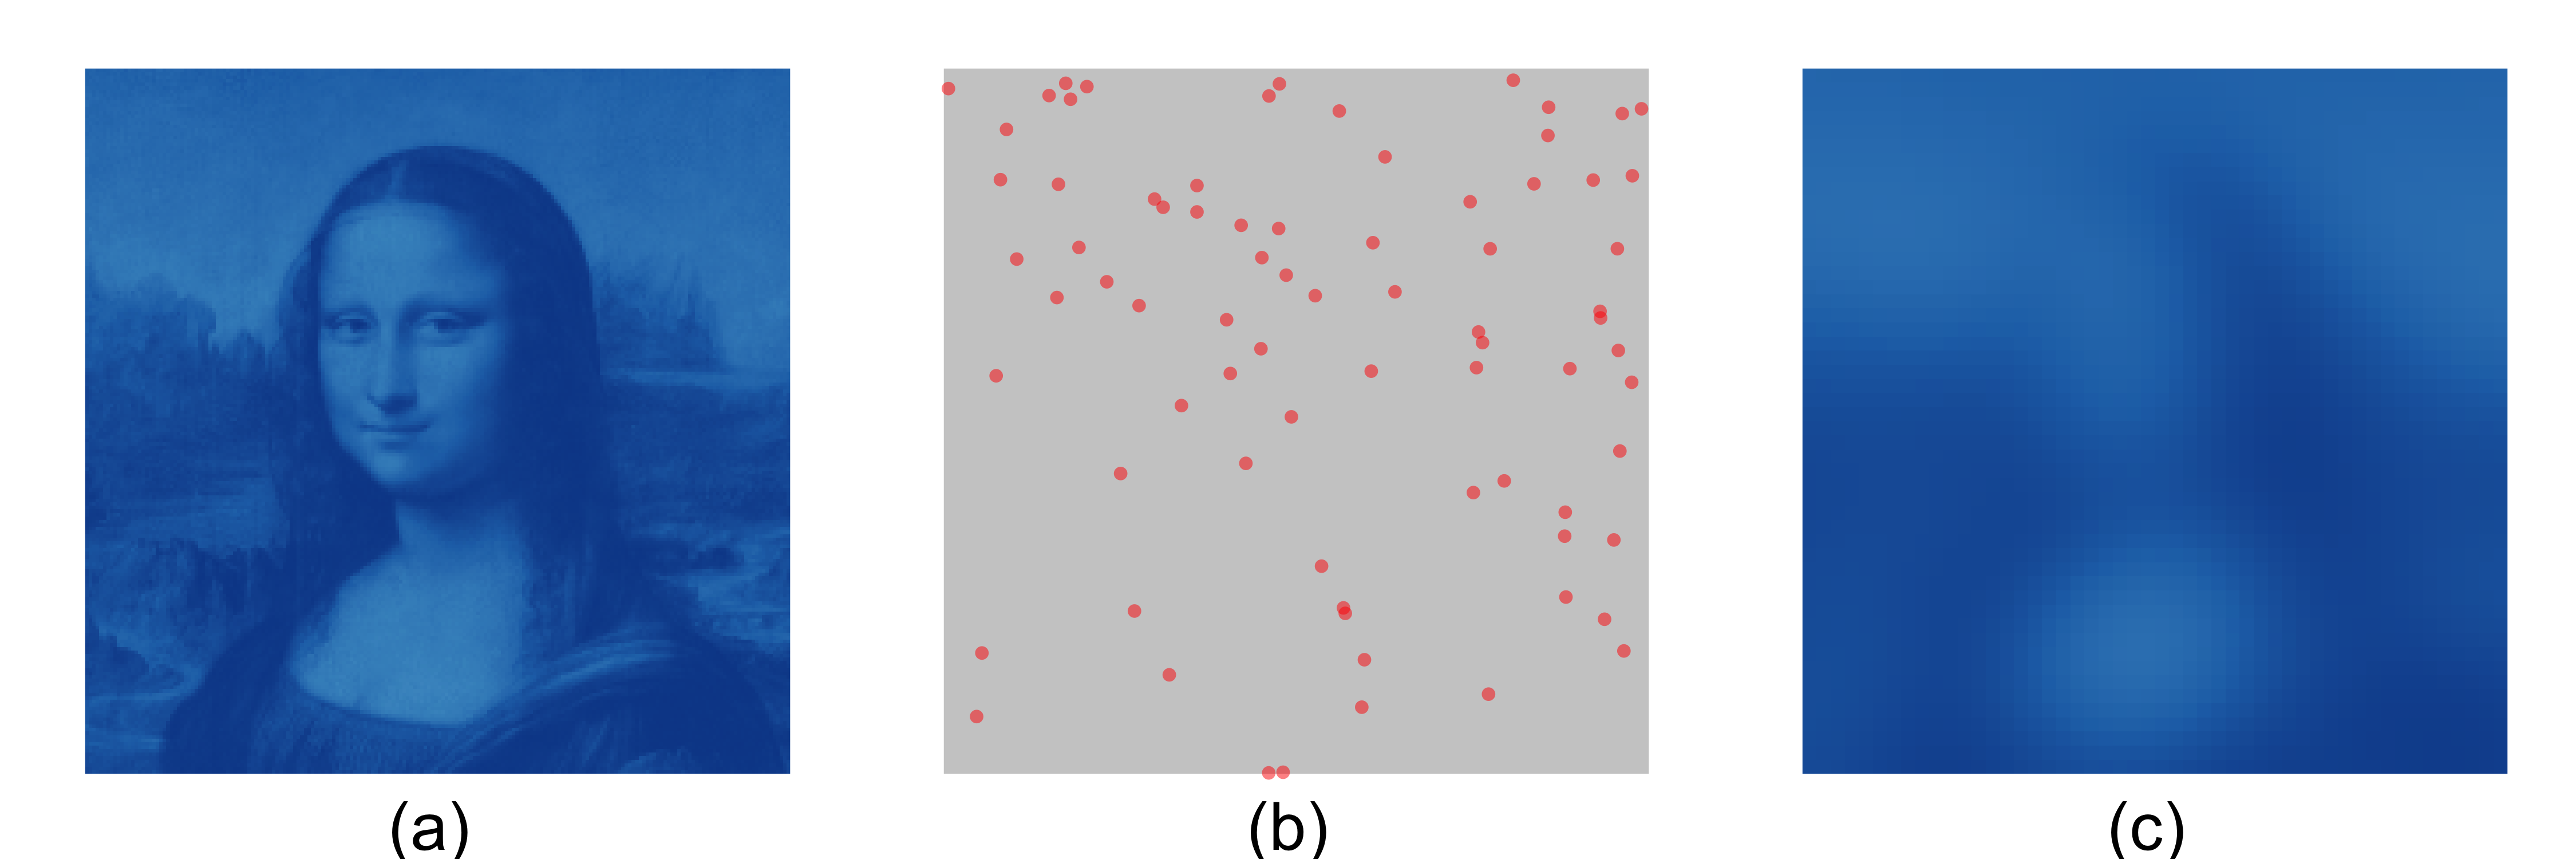
\includegraphics[width=1\textwidth]{mona_inputdata.png}
\caption{Input data for the Mona Lisa simulation study. Panel (a) shows a version of the Mona Lisa treated as an expected AC density surface. Panel (b) shows a single realization of 77 ACs generated from the surface in (a), while (c) shows a spatially-varying covariate that is correlated with true density, and which is used to estimate expected AC density surfaces.}
\label{mlinputs}
\end{figure}

We simulated capture histories from the population using a half-normal encounter rate function $\lambda(d) = \lambda_0\exp\{-d^2/(2\sigma^2)\}$, where $\sigma$ is a scale parameter determining how quickly the encounter rate decreases with $d$, the distance between the detector and the AC, and $\lambda_0$ is the expected encounter rate at a detector that is at the animal's AC ($d=0$). Arbitrarily defining the dimensions of the image to be $50\times 50$ units, we set $\sigma=4$ and used two different detector arrays: a $3\times3$ array centered at $x=18$ and $y=24$ (Figure~\ref{mona3x3}), and a $7\times 7$ array covering the entire image (Figure~\ref{mona7x7}). Note that the survey region is closed, in the sense that there are no detectable ACs beyond its borders. Both arrays had a fixed spacing of $2\sigma=8$ between detectors. The number of simulated detections of each animal at each detector was a Poisson random variable with expected value equal to the encounter rate function evaluated at the distance between the detector and AC. In order to illustrate how the two surfaces change with increasing sample sizes, we simulated capture histories with three different survey effort levels, obtained by varying $\lambda_0$ so that the average number of detections per detected individual was approximately two, four, or eight (corresponding to $\lambda_0=1.8, 5.2$, and $11.1$ for the $3\times 3$ grid, and $\lambda_0=0.7, 2.5$, and $5.5$ for the $7\times 7$ grid). This generated between 42 and 248 detections of between 21 and 33 individuals for the $3\times 3$ grid (Figure~\ref{mona3x3}), and between 68 and 674 detections of between 43 and 77 individuals for the $7\times 7$ grid (Figure~\ref{mona7x7}).

Parameter estimation by maximum likelihood SCR methods requires numerical integration of the likelihood, which is facilitated by defining a fine mesh of points at which the likelihood can be evaluated. This mesh, sometimes called the habitat mask, has the effect of discretizing continuous space into grid cells, with the mask points at the centers of the cells. We used a $50\times 50$ habitat mask i.e.\, a spacing of $1=\sigma/4$ between mask points. To estimate the predicted AC location surface, we assumed a model with constant density. 

To estimate an expected AC density surface, we generated a covariate by blurring the true AC density surface at the resolution of the habitat mask (Figure~\ref{mlinputs}(c)). Pixel intensities were rescaled after blurring so that the number of expected ACs remained the same as in the original surface (i.e., 80). Because it is based on true density, the covariate is very informative about the true densities, although the strength of the association is diluted by the blurring. We estimated an expected AC density surface assuming a model in which density was a function of covariate values. Note that, because density is parameterized with a log link but the blurred surface is obtained directly from the true density surface (so that $D(\mathbf{s})\approx x_1(\mathbf{s})$, with the degree of blurring determining the accuracy of approximation), covariate values were log-transformed to ensure the model was correctly specified.

Most of the examples of unclear or incorrect interpretations of density surfaces that we listed in the introduction are made using Bayesian methods. To show that correct interpretations do not depend on the inferential method used, models were fitted by both maximum likelihood, using the \texttt{secr} (v4.5.4) package \citep{secr:22} and Bayesian inference, using custom code written using the \texttt{NIMBLE} package \citep{deValpine:17, Turek:21} in R version 4.1.2. We report the maximum likelihood estimates here; the Bayesian estimates are not materially different and are reported in Web Appendix B, and are presented alongside plots of estimation uncertainty in Web Appendix C.

\section{Results}
The most striking features of the predicted AC location surfaces shown in Figure~\ref{mona3x3} (top row) are that (a) they do not recover the Mona Lisa in any recognizable way, (b) they predict flat density far from the array, (c) they become more ``spiked'' (density concentrated more closely around estimated AC locations) inside the array as sample size increases, and (d) the distance from the array at which the surface becomes flat increases as sample size increases. We discuss each of these features below

Regarding (a), predicted AC location surfaces are not designed to recover the expected density of ACs (the Mona Lisa image). They are designed to provide information about the locations of ACs in the surveyed animal population, given the capture histories observed. Point (b) is a consequence of this: because ACs far from the array are not detected, there is no information in the sample on their location other than that contained in the SCR estimate of mean density, and so all the model ``knows'' about ACs far from the array is that they occur in space at the estimated mean density of ACs. Point (c) and (d) are further consequences and essentially reflect the same phenomenon: as sample size increases, more information is collected on where ACs in the vicinity of the detectors are, and so the probability density of each predicted AC location contracts. Increasing survey effort increases sample size in two ways: animals already detected can be detected again, and animals not yet detected can be detected for the first time. Point (c) occurs because animals with ACs in the interior of the array tend to be detected most often. Point (d) occurs because increasing survey effort results in first detections of peripheral animals further away from the array, replacing their previous flat contributions to the surface with contributions that have some relief. This has the visual effect of pushing back the flat part of the surface and extending what is considered the periphery or ``in the vicinity'' of the array. 

Introducing covariates into the density model allowed us to recover features of the Mona Lisa across the entire image, not just near where detectors were located (Figure~\ref{mona3x3}, bottom row). Recovery may not be this good in reality -- we simulated our covariate to be strongly related to true density -- and extrapolation so far beyond the area where data was collected may be ill-advised in practice. Notwithstanding this, it is true in general that because the expected AC surface depends on the relationship between the covariate and density, the model uses estimates of this relationship obtained where it has lots of information (within the array) to infer density beyond the array. The inferred surface is also relatively insensitive to sample size.

The predicted AC location surface estimates in Figure~\ref{mona3x3} are misleading if interpreted as AC density plots, not because uncertainty about AC locations depends on sampling intensity, but because there are systematic spatial differences in this uncertainty (uncertainty is greater on the periphery of the array than inside it), and so spatial differences in AC density are confounded with spatial differences in uncertainty. Spatial differences in uncertainty are minimized if the survey region is closed and surveyed with high, even intensity (Figure~\ref{mona7x7}, top row). Predicted AC location surface estimates then provide a fair indication of AC distribution, although uncertainty will still be greater near the boundary of the survey region (because fewer detectors are within reach of an AC near the boundary than an AC that is well within the array). 

Where the survey region is not closed but has been evenly surveyed with a large, regular array, a similar effect can be achieved by restricting inference to the interior of the array, except that animals with ACs in the periphery outside the array will still make a contribution to the restricted surface. Note that, in contrast to the predicted AC location surfaces, the expected AC density estimates in Figure~\ref{mona7x7} (bottom row) are very similar to those in Figure~\ref{mona3x3}. 

\begin{figure}[htbp]
\centering
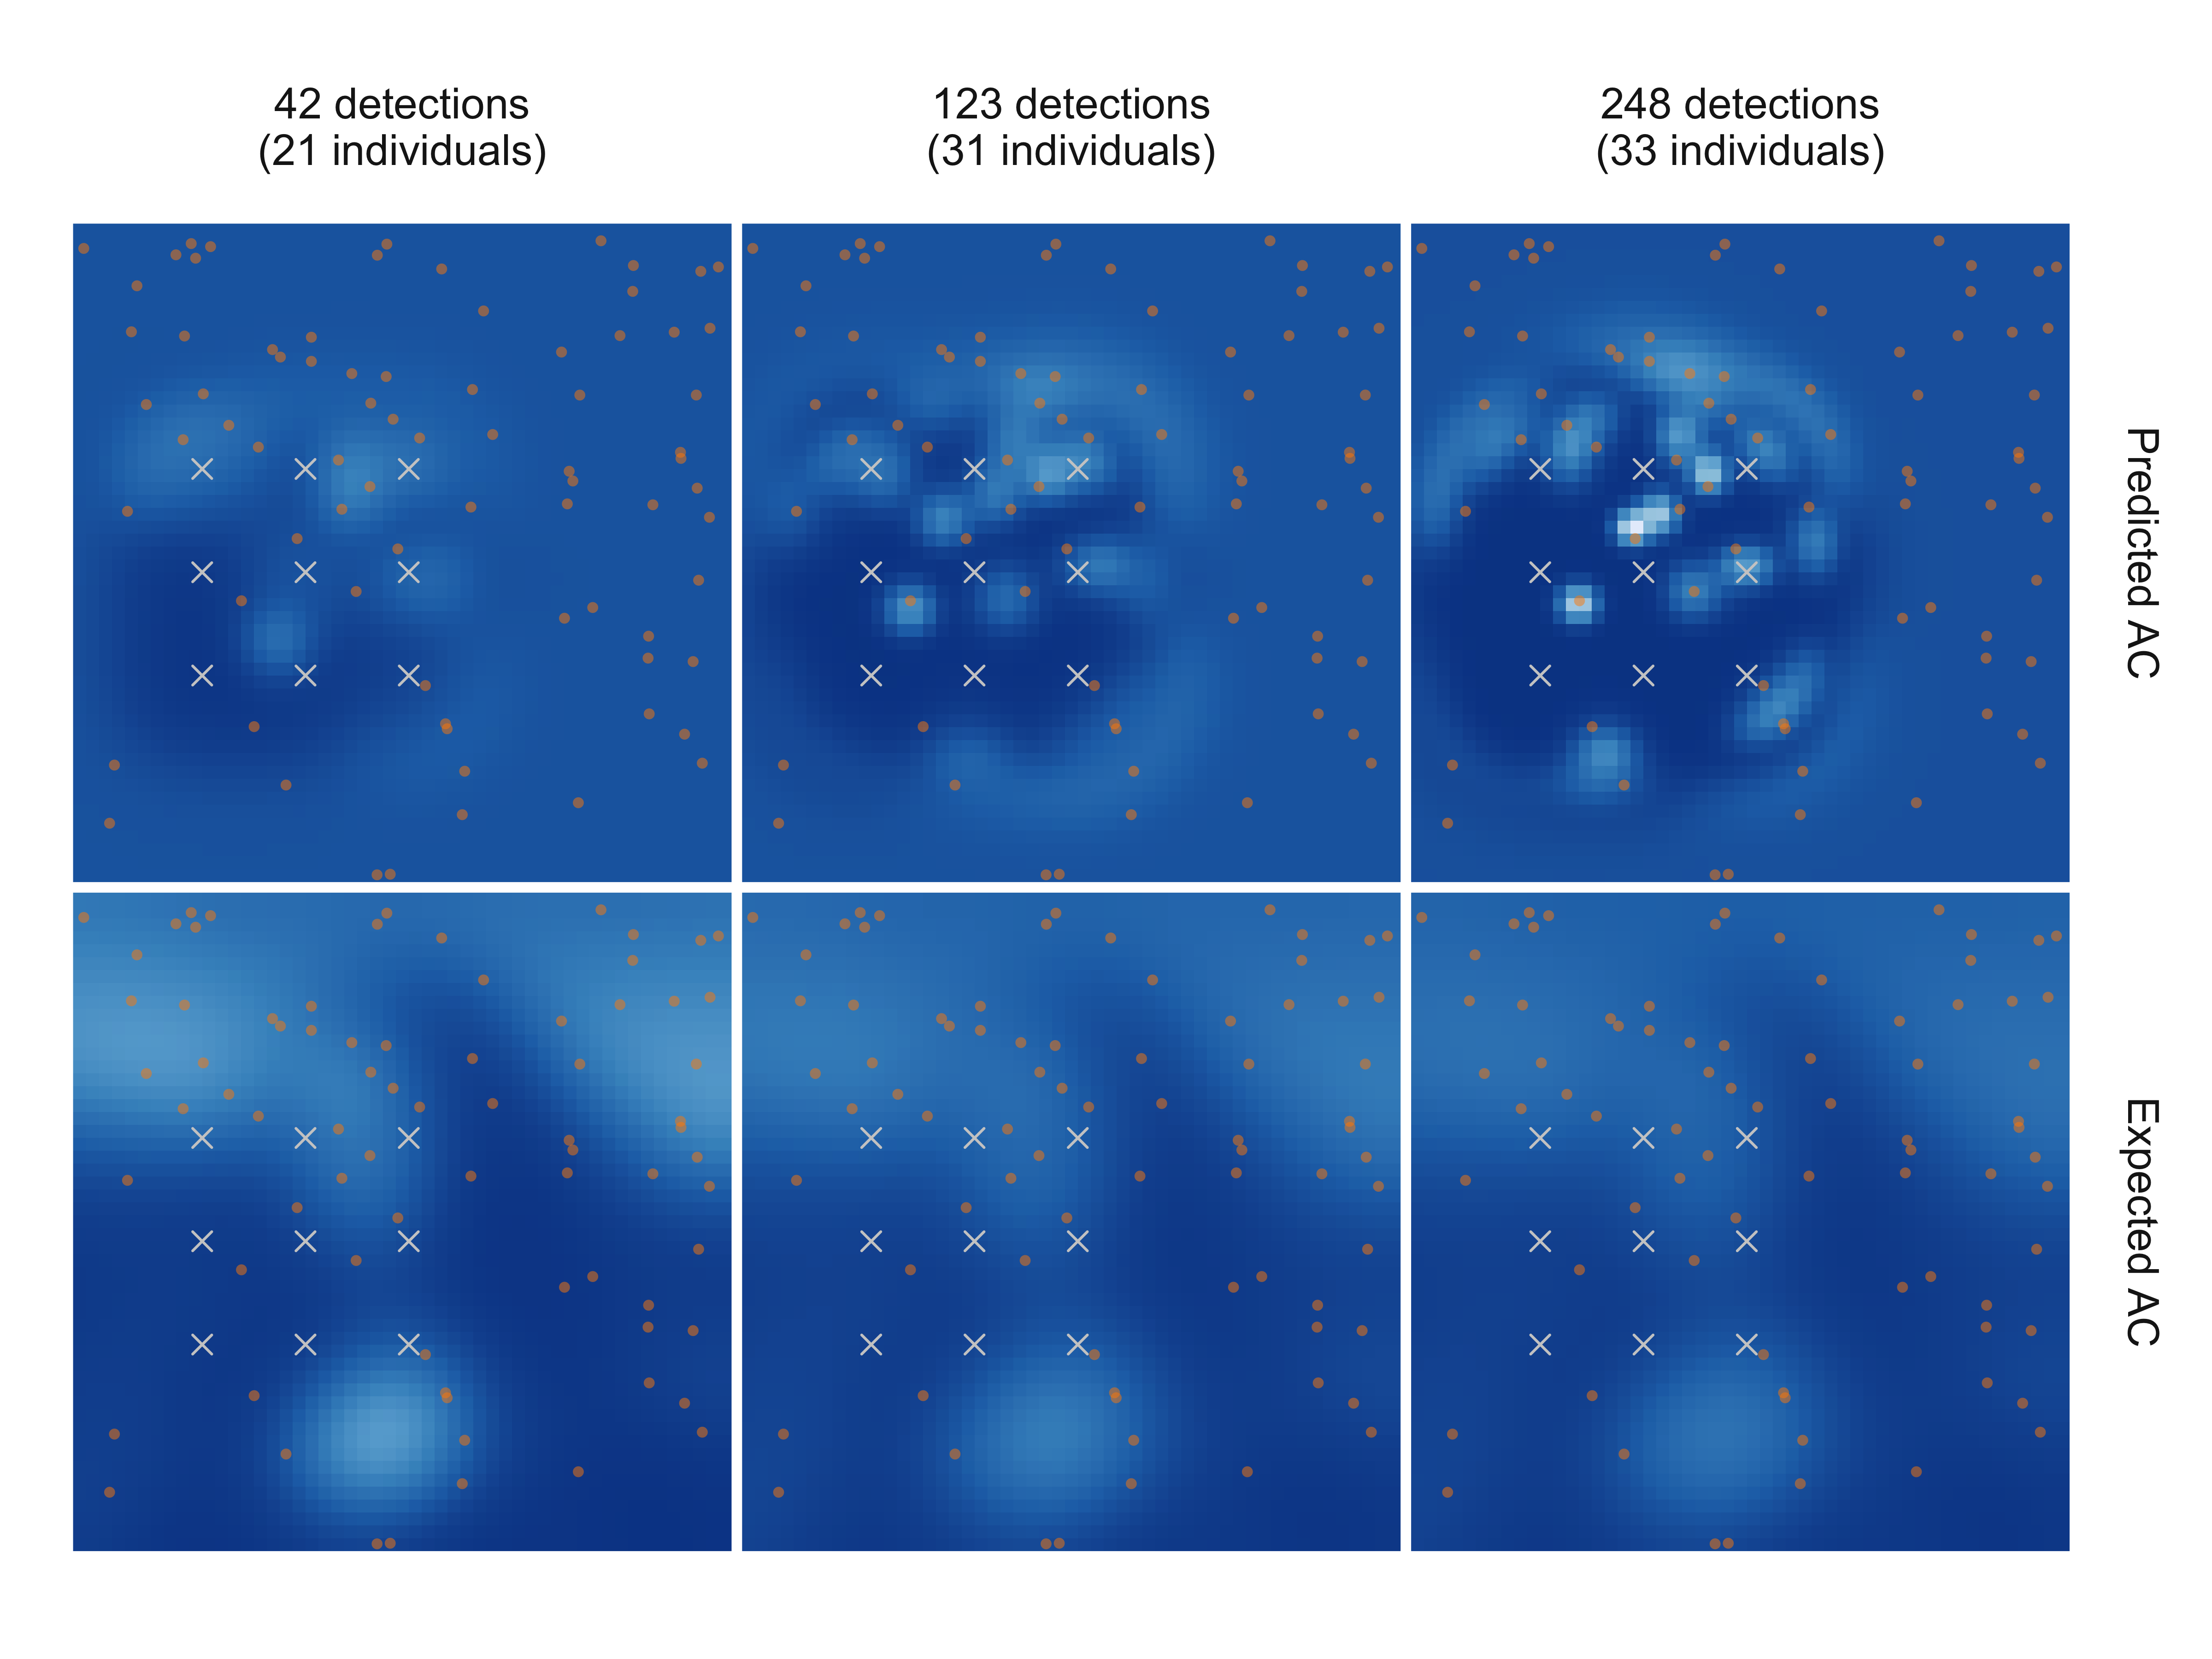
\includegraphics[width=1\textwidth]{mona_3x3.png}
\caption{Plots in the top row show predicted AC location surfaces estimated using the 3$\times$3 array indicated by grey crosses under three levels of survey effort. True AC locations are shown as orange dots. Plots in the bottom row show expected AC density surfaces estimated using a model in which density is a function of a simulated spatially-varying covariate (see Figure \ref{mlinputs}c). This figure appears in color in the electronic version of this article, and any mention of color refers to that version.}
\label{mona3x3}
\end{figure}


\begin{figure}[htbp]
\centering
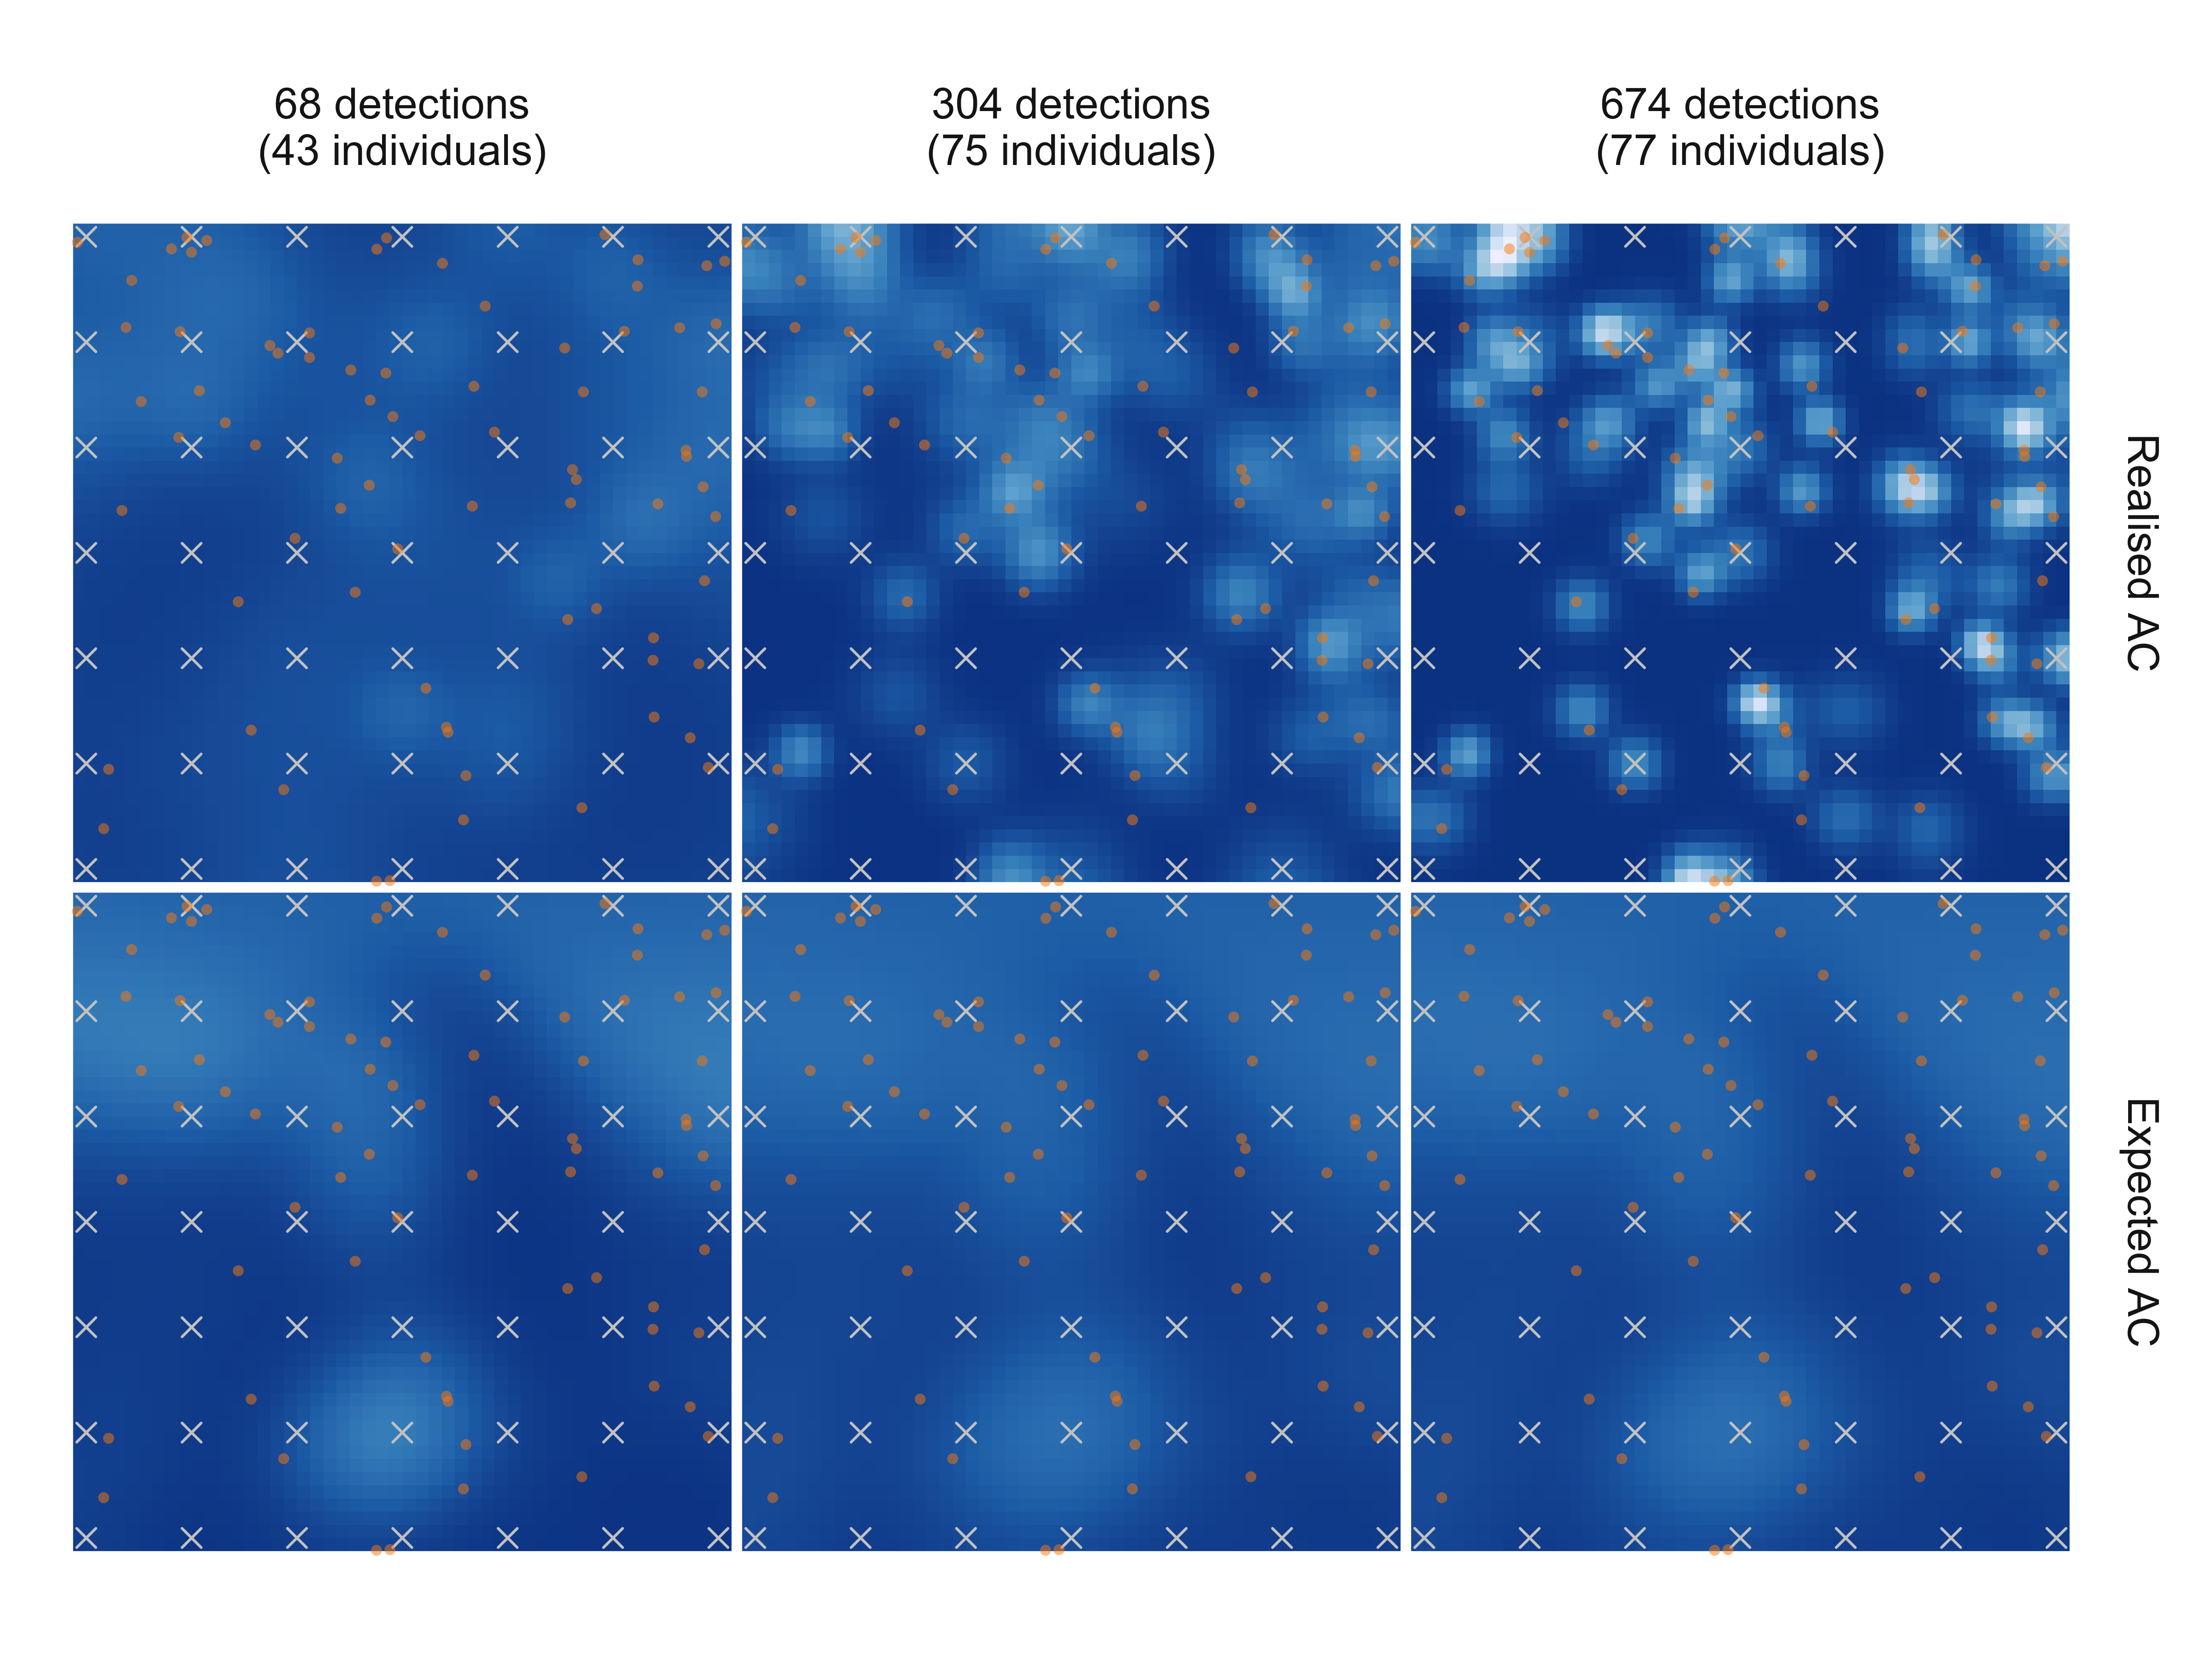
\includegraphics[width=1\textwidth]{mona_7x7.png}
\caption{Plots in the top row show predicted AC location surfaces estimated using the 7$\times$7 array indicated by grey crosses under three levels of survey effort. True AC locations are shown as orange dots. Plots in the bottom row show expected AC density surfaces estimated using a model in which density is a function of a simulated spatially-varying covariate (see Figure \ref{mlinputs}c). This figure appears in color in the electronic version of this article, and any mention of color refers to that version.}
\label{mona7x7}
\end{figure}

\section{Discussion and Conclusions} \label{discussion}
For most surveys, the predicted AC location surface produced from an SCR model cannot be interpreted as a density map in any meaningful biological or ecological way, because it depends heavily on factors related to the detection process that have nothing to do with the underlying AC intensity. 

Each AC PDF is a probabilistic prediction of the AC location of an animal given the capture history obtained for it by a survey, with the prediction obtained from a fitted SCR model. Although the capture history is associated with an individual animal, treating it as the density of AC locations for that animal ignores sampling variation in the possible capture histories that might have been obtained. This can be substantial for animals recorded only a few times by a survey. However, interpreting the predicted AC location surface as conditional on capture history is not at all straightforward because uncertainty depends on capture history in complicated ways that are difficult or impossible to discern from the produced surface once AC PDFs are summed up over individuals. 

The surfaces will always show less spatial variability far from the detector array than close to, or within it, whether the underlying intensity is less variable there or not. This point is clearly stated in \cite{Royle+al:13a}, who say (pp.\ 165--166) ``As we move away from `where the data live' (away from the detector array) we see that the density approaches the mean density. This is a property of the estimator as long as the detection function decreases sufficiently rapidly as a function of distance. ... predictions tend toward the global mean as the influence of data diminishes'', and also in \textit{secr} documentation warning that ``There are serious problems with the interpretation of such plots as `density surfaces'... the surface depends on sampling intensity, and as more data are added it will change shape systematically. Ultimately, the surface near the centre of a detector array becomes a set of spikes on a barren plain'' \citep{secr:22}. A survey that uses greater survey effort will produce a predicted AC location surface that has more spatial variability than a survey of exactly the same animals using lower effort. And the spatial variability moves with the array: move the array and the regions of high and low predicted values move with it, even though the true ACs are unchanged.

A useful metaphor here might be of SCR as a torch shining a light onto the true activity centers -- what you see depends on where you shine the torch (detector locations) and how brightly you shine it (survey effort). If you interpret the uniform darkness outside of the beam to mean that everything outside the beam is the same, you fundamentally misunderstand the nature of torches and will draw fundamentally incorrect conclusions.

When considering predicted AC locations, SCR models answer the question ``where is an animal with {\it this} spatial capture history likely to have its activity center?'' The answer is always contingent on where detectors are located - because the capture history depends on where the detectors are located. This is the case regardless of whether one works in a Bayesian or frequentist framework. The same is true of the predicted AC location surface, which simply sums estimated AC PDFs across animals, and will also be true for any downstream analyses that make use of the predicted AC location surface e.g.\ density-weighted connectivity \citep{Morin2017}. 

Uncertainty about the location of an animal's AC is affected by the number of times it is detected and the number of detectors it is detected at (and to some extent by the spatial configuration of those detectors). These quantities tend to be larger, and so uncertainty less, for animals whose ACs are within reach of more detectors i.e.\ for animals whose ACs are well inside the detector array. Concerns about spatial differences in uncertainty are diminished when the surveyed area is large and surveyed with high and even detector intensity, and under these conditions the predicted AC location surface provides a reasonable reflection of the spatial distribution of ACs, particuarly within the array. But these conditions are not likely to hold in many SCR studies.

To extend the metaphor, a torch beam's does not abruptly change from bright to dark. At the periphery of the beam (near the extent of the array) objects become increasingly difficult to see. Increasing the brightness of the torch makes everything within the beam easier to see, but also pushes back the periphery of the beam. Drawing a line at which the torch can no longer be trusted is to some extent arbitrary. 

An apparent way of enhancing the interpretability of predicted AC location surfaces is to present accompanying surfaces that convey the uncertainty in the predicted AC location estimate in each pixel. While measures quantifying the uncertainty in AC density surface estimates can be easily computed, we found that these were ineffective in communicating the systematic spatial differences in locational uncertainty that affect predicted AC location surfaces (Web Appendix C). Pixel-specific standard deviations were strongly correlated with the predicted AC density in that pixel, and so conveyed much the same pattern as the AC density surfaces. Coefficients of variation were highest in pixels with near-zero densities. Both of these measures indicated that uncertainty was highest within the array. In addition uncertainty in predicted AC location surface estimates was sensitive to the arbitrary choice of grid cell size, with higher precision (lower standard deviations, for example) obtained with larger cell sizes. 

There is a way of using SCR so that parameter estimates can be interpreted in a biologically or ecologically meaningful way, and this is by modeling the intensity of the underlying process as a function of covariates. Covariates allow one to see beyond the spatial extent of the array (see bottom rows of Figures~\ref{mona3x3} and \ref{mona7x7}), provided that the relationship between covariate and response is a good one, and that detectors cover a sufficient range of covariate values to estimate that relationship well. In principle spatial trend models are capable of retrieving patterns without covariates other than spatial coordinates, though usually environmental covariates are preferred for interpretability. The resulting surfaces show the (estimated) intensity of the underlying process assumed to generate activity centers. These expected densities will be highest where covariates are most favorable. Using covariate models, and associated model-based inference, is not without issues -- there is a danger of extrapolating the density surface beyond the range of covariates around the detectors, particularly with a log link function, and the relationship with density and covariate is assumed to be the same everywhere as it is around the detectors. Notwithstanding this, expected AC density surfaces are no longer strongly tied to one particular realization of the Poisson process or to where detectors are placed.

Ultimately, the appropriate density surface to use depends on the aims of the researcher. We have argued that the predicted AC location surface should not be used, because of the strong dependence on detector location and survey effort. But if the goal is to identify the ACs of {\it some} animals currently in the study region (and it does not matter which ones) then it may well be an efficient way of locating these, especially in the interior of large survey regions sampled evenly and with high effort. If the goal is to estimate where animals (not just the ones detected by the current survey) are likely to have activity centers, then the expected AC density surface, with density a function of covariates, should be used.

\section*{Acknowledgements}

This work was part-funded by the Royal Society of New Zealand through Marsden grant UOA-1929. We thank two anonymous reviewers and the associate editor for their helpful comments.

\section*{Data Availability Statement}
All code and output are available at https:/doi.org/10.5281/zenodo.10069782. This provides a permanent link to the version of the repository https:/github.com/iandurbach/monalisa used to generate the results in this paper.

\bibliographystyle{biom}
\bibliography{monalisa}

\section*{Supplementary Materials}
Web Appendices referenced in Sections 2 and 3 and Figures referenced in Sections 2 and 4, are available with this paper at the Biometrics website on Oxford Academic.

\end{document}


%%% Local Variables:
%%% mode: latex
%%% TeX-master: t
%%% End:
